\documentclass[12pt]{article}
\usepackage[utf8]{inputenc}
\usepackage[spanish]{babel}
\usepackage[pdftex]{graphicx}
\usepackage{float}
\usepackage{booktabs}
\usepackage[table,xcdraw]{xcolor}
\usepackage{ltxtable}
\begin{document}
\begin{titlepage}

\begin{minipage}{2.6cm}

\includegraphics[width=\textwidth]{fceia.pdf}
\end{minipage}
\hfill
%
\begin{minipage}{6cm}
\begin{center}
\normalsize{Universidad Nacional de Rosario\\
Facultad de Ciencias Exactas,\\
Ingeniería y Agrimensura\\}
\end{center}
\end{minipage}
\hspace{0.5cm}
\hfill
\begin{minipage}{2.6cm}

\includegraphics[width=\textwidth]{unr.pdf}
\end{minipage}

\vspace{0.5cm}

\begin{center}
\normalsize{\sc R-222 Arquitectura del Computador}\\
\vspace{0.5cm}
\large{Trabajo Práctico Final}\\

\Large{\bf Compilador y Máquina Virtual para arquitectura MIPS}\\
\vspace{5cm}

\normalsize
 Román Castellarin\\
Lisandro Maselli\\
Juan Ignacio Suarez\\

\vspace*{0.5cm}
\small{11 de Abril de 2018}


\end{center}
\end{titlepage}
\newpage
\section{Introducción}
El proyecto aquí presentado consistió en la investigación de las arquitecturas MIPS, para el consecuente desarrollo de una máquina virtual y un compilador que en conjunto permiten ejecutar código assembly directamente.

El proyecto consta de 2 partes:
\begin{itemize}
\item Un compilador (compuesto de un lexer + parser) que toma código assembly para MIPS y genera un archivo ejecutable para la máquina virtual.
\item Una máquina virtual que toma el archivo generado y lo ejecuta.
\end{itemize}    

\section{Arquitectura MIPS}
En arquitectura computacional, RISC (Reduced Instruction Set Computer) es un tipo de diseño de CPU generalmente utilizado en microprocesadores
o microcontroladores con las siguientes características fundamentales:
\begin{itemize}
\item Reducida cantidad de ciclos por instrucción (CPI)
\item Instrucciones de tamaño fijo y presentadas en un reducido número de formatos.
\item Sólo las instrucciones especificas de carga y almacenamiento acceden a la memoria de datos.
\end{itemize}



Para este trabajo elegimos emular  la arquitectura de MIPS I, la cual consta con estas características  principales :
\begin{itemize}
\item Ancho de palabra y tamaño de los buses : 32 bits
\item  Tamaño de los datos en las instrucciones:
	\begin{itemize}
	\item Byte (b): 8 bits
	\item Halfword (h): 16 bits
	\item Word (w): 32 bits
	\item Doubleword (d): 64 bits
	\end{itemize}
 \item Arquitectura de carga / almacenamiento:
 	\begin{itemize}
 	\item Antes de ser utilizado en una instrucción aritmética, todo dato debe
 	ser cargado previamente en un registro de propósito general.
 	\item Instrucciones aritméticas con 3 operandos (2 sources y 1 destino) de 32 bits en registros.
 	\end{itemize} 
\end{itemize}
\subsection{Registros}
En MIPS los registros \$0 a \$31 son de propósito general y pueden emplearse
para contener datos o punteros.\\
Existe un convenio que dota de pseudónimos y usos determinados a todos los
registros del MIPS:

\begin{table}[H]
\centering
	\begin{tabular}{@{}lll@{}}
	\toprule
	\multicolumn{1}{c}{Nombre} & Número & Uso          \\ \midrule
	\$zero                & 0 & constante 0 (sólo lectura). \\
	\$at                  & 1 & uso interno del ensamblador al decodificar pseudoinstrucciones. \\
	\$v0 - \$v1       & 2-3 & valores de retorno de subrutinas. \\
	\$a0 - \$a3      & 4-7 & argumentos para subrutinas. \\
	\$t0 - \$t9      & 8-15, 24-25 & variables temporales. \\   
	\$k0 - \$k1     & 26-27 & reservado para el uso del kernel del SO.\\   
	\$gp                 & 28 & puntero de tabla de datos globales.\\
	\$sp                & 29 & puntero de pila.\\
	\$fp                 & 30 & puntero de marco. \\
	\$ra                 & 31 & dirección de retorno (usado implícitamente por instrucción jal).
	\end{tabular}%
\end{table}
Además cuenta con con 2 registros de 32 bits especiales  llamados HI y LO, que sirven
para almacenar los resultados de la multiplicación/división y operaciones de transferencia de datos.
\subsection{Memoria}
La dirección física de la memoria de instrucciones, en modo usuario, empieza en la dirección 0x400000 y termina en 0x0FFFFFFF. Mientras que la dirección de la memoria
de datos, en modo usuario, empieza en la 0x10000000 y termina en la 0x7FFFFFFF.
\begin{center}
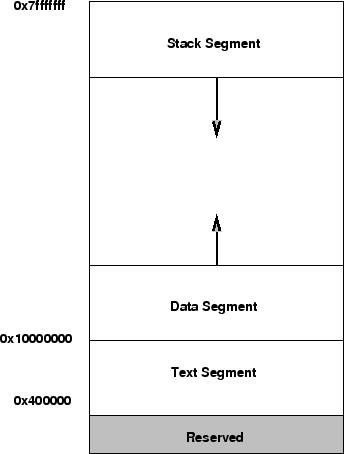
\includegraphics[height=\dimexpr\pagegoal-\pagetotal-\baselineskip\relax,width=\textwidth,keepaspectratio]{gmemory.png}
\end{center}
MIPS tiene restricciones de acceso a memoria porque utiliza el byte como mínima unidad con dirección:
\begin{itemize}
\item Las palabras tienen que empezar en una dirección múltiplo de 4.
\item Las medias palabras tiene que empezar en una dirección múltiplo de 2.
\end{itemize}
\subsection{Instrucciones}
El conjunto de instrucciones permite realizar instrucciones de carga y almacenamiento
desde y hacia memoria, tiene capacidad de desarrollar programas que resuelven problemas aritméticos y lógicos, y ofrece la posibilidad de controlar el flujo de la ejecución del programa mediante instrucciones de comparación y salto.
Una breve clasificación sería:
\begin{itemize}
\item Instrucciones aritméticas.
\item Instrucciones lógicas.
\item Instrucciones de salto condicional.
\end{itemize}
También se pueden clasificar en función de los elementos que utilizan (banco de registros, memoria de datos, ALU).Cada uno de los componentes que utiliza la instrucción se debe especificar en una serie de bits. Los distintos tipos de instrucciones
constan de diferentes tamaños para los espacios reservados para esos bits, es decir, utilizan diferentes formatos para codificar sus campos.\\
En MIPS R2000 se distinguen tres tipos de formatos de instrucción:
\begin{itemize}
\item Formato R o de tipo registro
\item Formato I o de tipo inmediato.
\item Formato J o de salto incondicional
\end{itemize}
\begin{center}
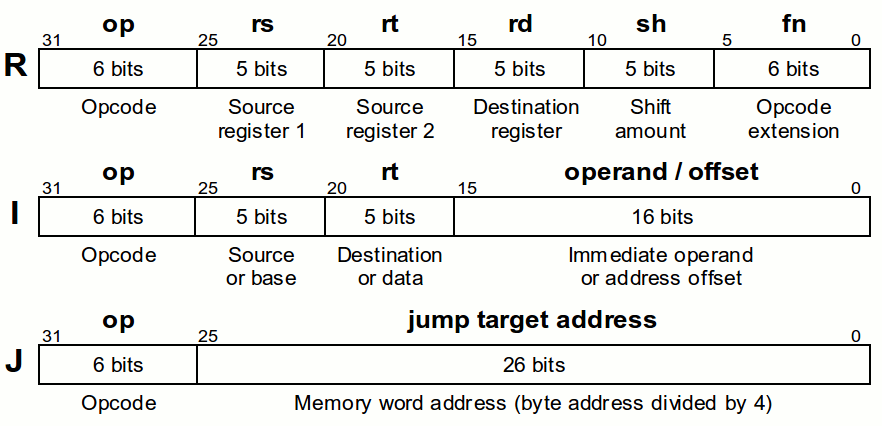
\includegraphics[width=\textwidth,keepaspectratio]{formatos.png}
\end{center}

\LTXtable{\textwidth}{instructions_table}
    
\section{Compilador}
\subsection{Formato ejecutable .mips}

En un archivo compilado se puede encontrar mucha más información que las instrucciones del programa que codifica, por lo tanto, su formato no sólo depende de la arquitectura, sino además del sistema operativo.

Nuestra MV utiliza el siguiente formato -creado por nosotros- al cual le asignamos extensión .mips.
\\

ARCHIVO EJECUTABLE
\begin{itemize}
\item Header (12 bytes):
	\begin{itemize}
    		\item 4B : tamaño del segmento de datos (en bytes)

  		\item 4B : tamaño del segmento de texto (en bytes)

    		\item 4B : direccion del main
	\end{itemize}
\item Segmento de Datos (tamaño dado por la cabecera):

    Las direcciones comienzan en 0x10000000

\item Segmento de Texto (tamaño dado por la cabecera):

    Las direcciones comienzan en 0x400000
\end{itemize}
\textit{Ver sección MV para mayor información sobre el mapeo de memoria.}

\subsection{Lexer}

\subsubsection{Introducción}

El primer paso para la compilación consiste en un Analizador léxico (también llamado Analizador lexicográfico, Scanner o Lexer), que nos permitirá reconocer en orden cada instrucción o directiva del código fuente, donde luego produciremos como salida una secuencia de tokens (componentes léxicos).

En resumen, nuestro Lexer recibe el código fuente como entrada y produce una secuencia de tokens como salida, para luego poder analizar el programa sintácticamente.
Para esto utilizaremos un analizador léxico llamado Flex (fast lexical analyzer generator).

\subsubsection{Funcionamiento}
El funcionamiento de Flex es relativamente simple. Dada una lista de matchings posibles y token único asignado a cada match, devuelve el token del match siguiente más grande posible. Por ejemplo:

\begin{verbatim}
".asciiz"	{ return T_ASCIIZ_DIRECTIVE; }
\end{verbatim}

Devolverá el token asociado cuando encuentre una directiva asciiz. Notar que el Lexer tiene funcionalidades más poderosas como expresiones regulares, que mencionamos a continuación.

\subsubsection{Características}
Nuestro Lexer usa expresiones regulares para reconocer estructuras léxicas más complicadas como etiquetas, números hexadecimales/decimales, strings y datos de tipo char. Con la sintaxis de flex, algunas de las expresiones regulares que usamos son:

\begin{verbatim}
    id 			[a-zA-Z_][a-zA-Z0-9_]*
\end{verbatim}

Esta expresión nos indica que un id comienza con un caracter entre a-z, A-Z ó '\_', y a continuación le sigue una cantidad indeterminada de caracteres entre a-z, A-Z, 0-9 ó '\_'.

\begin{verbatim}
    char  		(\\['"\?\\abfenrtv])|([a-zA-Z0-9])
\end{verbatim}

Según esta definición, un char válido es algún caracter entre a-z, A-Z, 0-9 ó un caracter especial escapeado, como \verb!\n!. Luego utilizamos esta definición en otra más compleja:

\begin{verbatim}
    hexnumber 	(0[xX][0-9a-fA-F]+)|(-?[0-9]+)|('{char}')
\end{verbatim}

Donde aceptamos un número en formato hexadecimal, en decimal o como char encerrado entre comillas simples. De manera similar se pueden construir expresiones más grandes para reconocer otros tipos de expresiones.

\subsection{Parser}

Para traducir el codigo MIPS a sus expresiones en binario, el parser recibe secuencialmente los tokens producidos por el lexer.
Internamente posee dos estructuras de control que le permite llevar a cabo la operacion:
\begin{itemize}
	\item Un map en el que lleva las direcciones de cada etiqueta.
	\item Contadores que llevan la direccion del segmento de datos y del segmento de codigo actual.
\end{itemize}
De esta forma el parser es capaz de saber en que segmento y dirección  se encuentra.Para traducir las instrucciones,
cada tokens es organizado dependiendo el formato de la instrucción y que tipo de parametros que recibe, lo cual le permite analizar
semanticamente la sentencia y traducirla.


\subsection{Problemas encontrados}

\begin{itemize}

\item	El análisis sintáctico se produce en orden linealmente desde el inicio del archivo hasta el final. Esto produce que ciertas instrucciones no puedan ser procesadas en determinado instante pues referencian etiquetas que aún no han sido procesadas. Para solucionar este problema el compilador hace dos pasadas: en la primera sólo calcula la dirección de memoria de cada etiqueta, y en la segunda puede procesar cada instrucción sin problemas.

\item    Encontramos un problema de compatibilidad dependiendo el modo en el que se accede a la escritura del ejecutable. Abriendo el archivo en modo texto resulta en un output distinto bajo Linux y Windows. Para obtener el mismo resultado en ambas plataformas se debe abrir como archivo binario.
    
\end{itemize}

   
\section{Máquina virtual}
\subsection{Introducción}
para emular el procesador vamos a mantener todos los registros en memoria y a
medida que se interpretan las instrucciones estos van modificándose.
para eso definimos a los registros como un array de 32 enteros de 32 bits
y 3 variables de enteros de 32 bits para  los registros LO, HI y PC.

la interpretación de las instrucciones se lleva a cabo primero decodificando
estas y mapeando su significado a una función respectiva.
\subsection{Mini SO ficticio}
\subsubsection{Mapeo de memoria}
Nuestra maquina provee a los programas que ejecuta direcciones virtuales,
cada vez que un programa desea realizar un acceso a memoria, ya sea para lectura o escritura,
el SO intercepta dicha dirección y la traduce a direcciones reales. 

\begin{center}
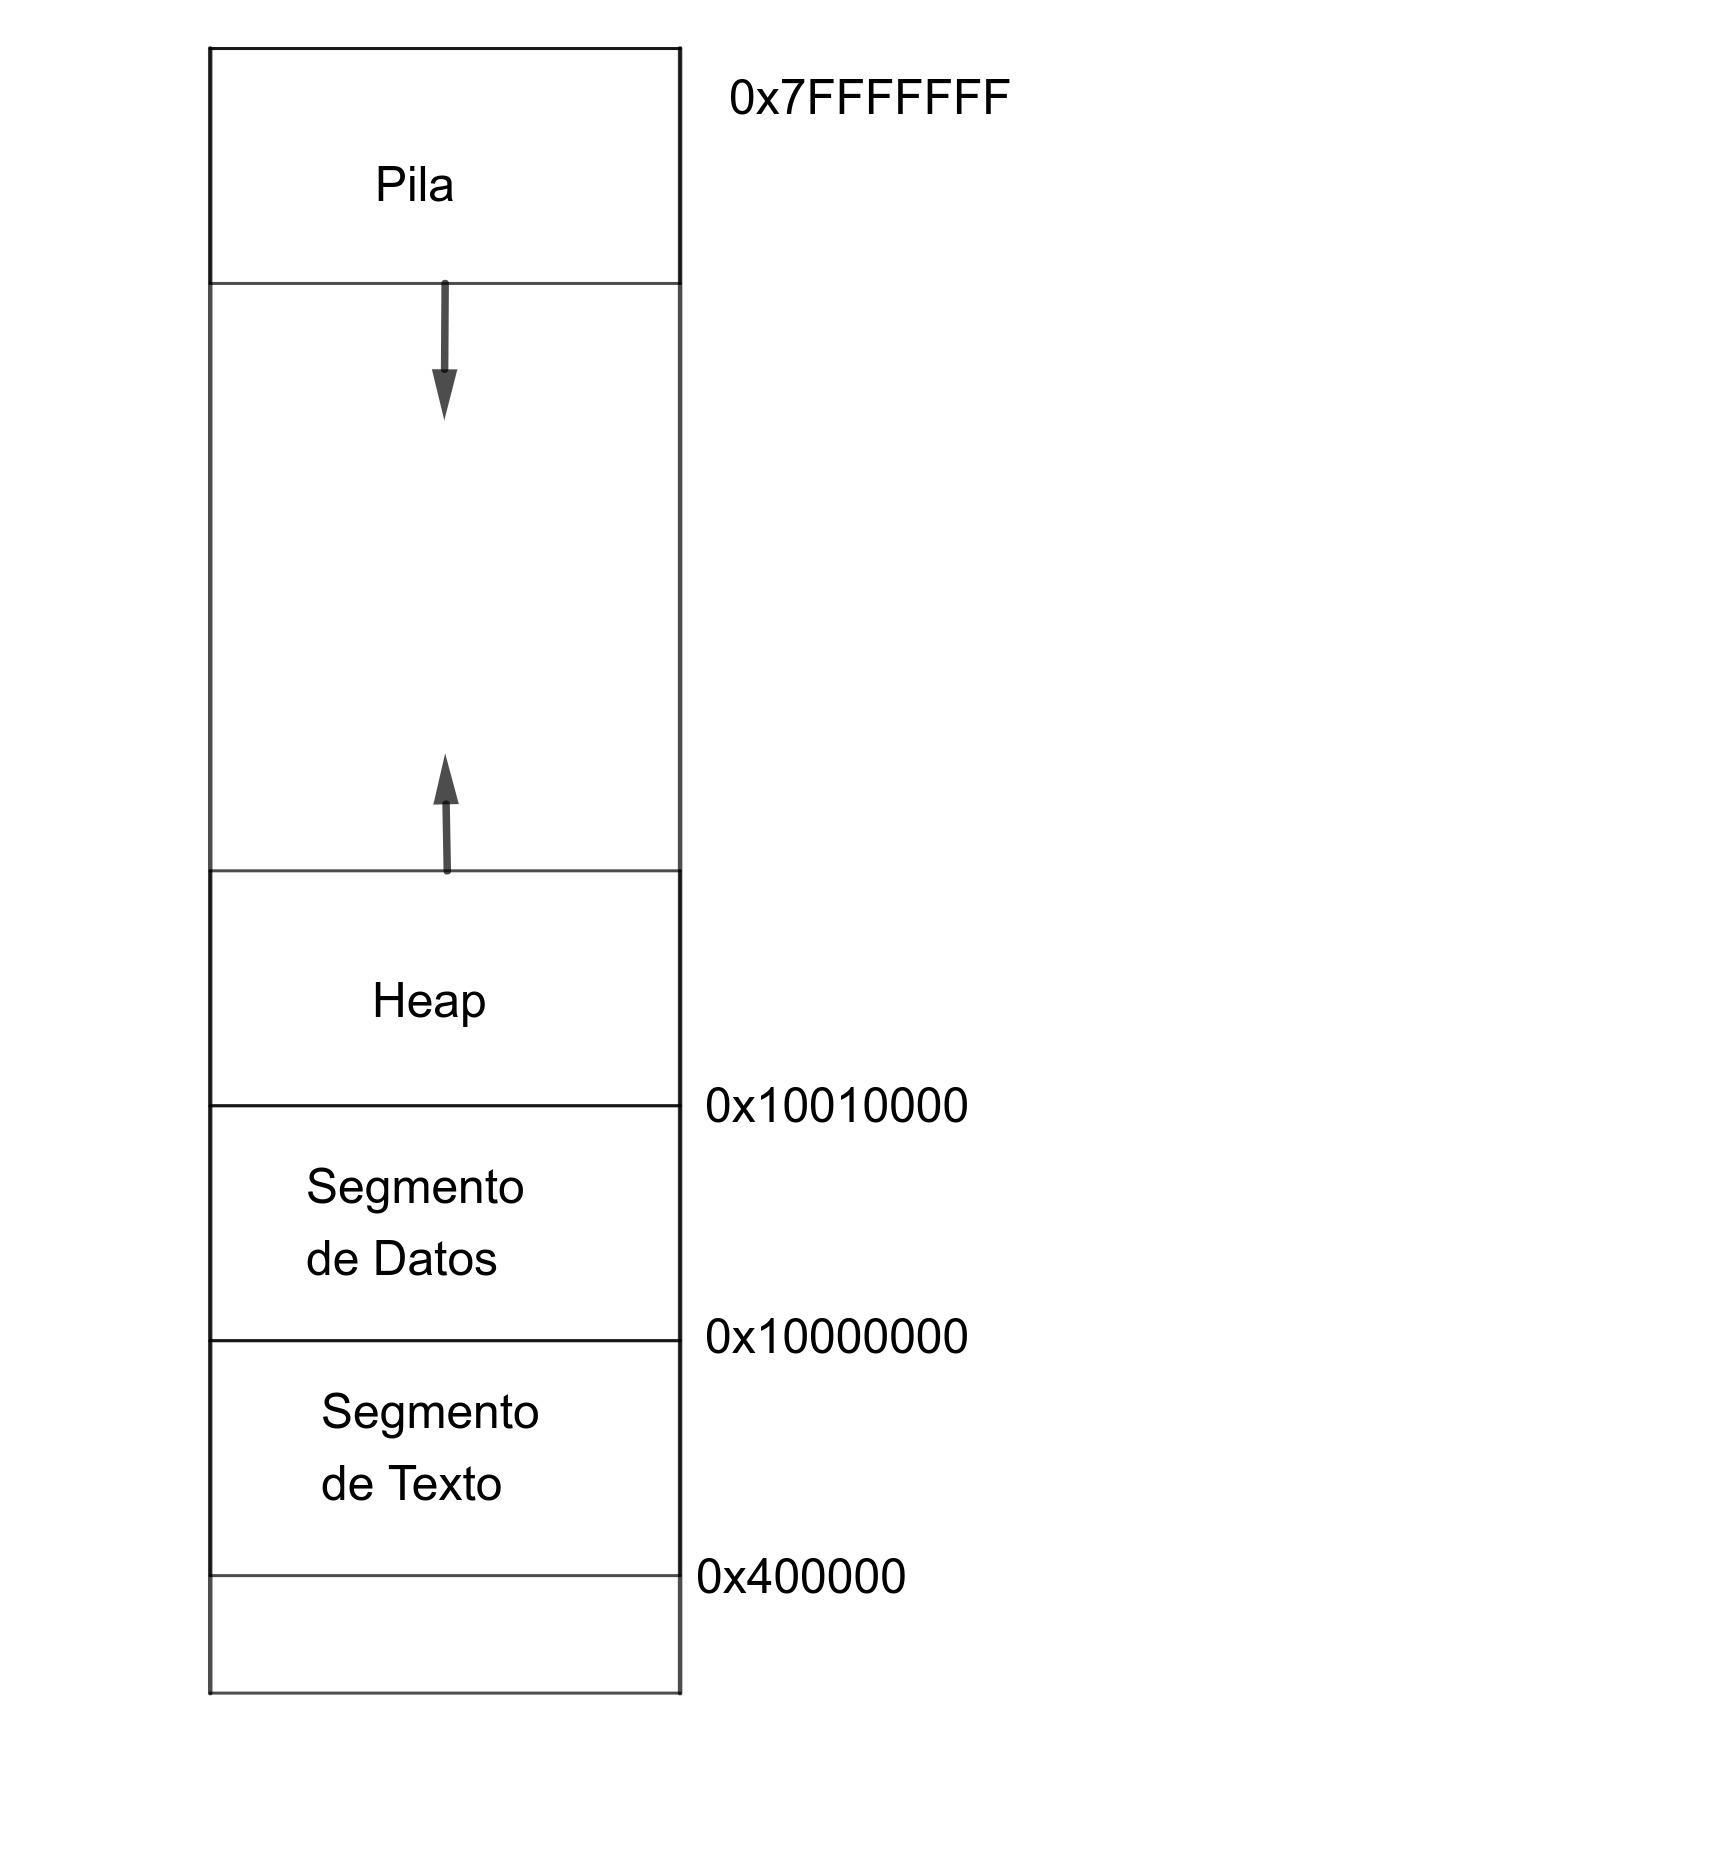
\includegraphics[height=10cm]{mdetails.png}
\end{center}

\begin{itemize}
\item El segmento de texto comienza en 0x400000
\item El segmento de datos estático comienza en 0x10000000
\item La memoria dinámica comienza en 0x10010000
\item La pila termina en 0x7FFFFFFC
\end{itemize}
\subsubsection{Syscalls provistas}
Tambien dotamos de primitivas a nuestro S.O. para poder realizar programas con mayor soltura.
Las siguientes syscalls han sido diseñadas e implementadas:
\begin{table}[H]
\centering
\begin{tabular}{@{}llc@{}}
\toprule
\multicolumn{1}{c}{Nombre} & Argumento/Retorno & Numero \\ \midrule
SC\_PRINT\_INTEGER & \texttt{\$a0} - entero a imprimir                    & 1      \\
SC\_PRINT\_FLOAT    & \texttt{\$f12} - float a imprimir                   & 2      \\
SC\_PRINT\_DOUBLE   & \texttt{\$f12-13} - double a imprimir                    & 3      \\
SC\_PRINT\_STRING   & \texttt{\$a0} - puntero a string a imprimir                   & 4      \\
SC\_READ\_INTEGER   & \texttt{\$v0} - entero leído                  & 5      \\
SC\_READ\_FLOAT     & \texttt{\$f0} - float leído                  & 6      \\
SC\_READ\_DOUBLE    & \texttt{\$f0-1} - double leído                   & 7      \\
SC\_READ\_STRING    & \texttt{\$a0} - dir. donde guardar el string, \texttt{\$a1} - max.long.                  & 8      \\
SC\_MALLOC          & \texttt{\$a0} - bytes solicitados, \texttt{\$v0} - dirección otorgada            & 9      \\
SC\_EXIT            &           & 10      \\
SC\_PRINT\_CHAR     & \texttt{\$a0} - char a imprimir                 & 11      \\
SC\_READ\_CHAR      & \texttt{\$v0} - char leído                & 12      \\
\end{tabular}%
\end{table}

Para llamar a alguna de estas llamadas al sistema, es necesario guardar el numero en
\texttt{\$v0} y luego invocar la instrucción \texttt{syscall}.


\subsection{Modulos}
\subsubsection{Syscalls}
Este modulo se encarga de la implementacion de las llamadas al sistema.

La mayoría de las syscalls son simplemente \textit{wrappers} de \texttt{scanf} y \texttt{printf}, aunque \texttt{malloc} tiene una implementacion propia en el modulo \texttt{memory.h}. 




\subsubsection{Simulator}

Este modulo contiene las funciones necesarias para inicializar y resetar la maquina virtual. Ademas, implementa un pequeño \textit{shell} que permitirá correr los programas con mayor control sobre ellos. En particular, este modulo maneja los breakpoints. 

Las operaciones soportadas por el shell  son las siguientes:

\begin{table}[H]
\hskip-2.0cm
\begin{tabular}{@{}cll@{}}
\toprule
\multicolumn{1}{c}{Atajo} & Nombre                                                       & Acción                                                                        \\ \midrule
h                         & help                                                         & muestra esta tabla de comandos.                                               \\
l                         & load \textless nombre archivo\textgreater                  & abre el archivo indicado.                                                     \\
n                         & step                                                         & realiza un paso en la simulación.                                             \\
n                         & step \textless n\textgreater                                  & realiza n pasos de la simulación.                                             \\
r                         & run                                                          & continúa la ejecución hasta un punto de interrupción.                         \\
i                         & init                                                         & inicializa la máquina virtual para una segunda ejecución.                     \\
w                         & where                                                        & imprime el valor actual del reg. PC y la instrucción apuntada.    \\
b                         & break \textless lista de dirs\textgreater              & coloca puntos de interrupción en las dir. especificadas.               \\
b                         & break                                                        & muestra todos los puntos de interrupción actuales.                            \\
c                         & clear \textless lista de dirs\textgreater              & borra todos los puntos de interrupción de las direcciones indicadas.          \\
c                         & clear                                                        & borra todos los puntos de interrupción.                                       \\
g                         & ignore \textless n\textgreater                                & ignora n puntos de interrupción consecutivos.                                 \\
j                         & jump \textless dirección\textgreater                          & modifica el registro PC para que apunte a la dirección seleccionada.          \\
s                         & set \textless registro\textgreater \textless\%i\textgreater   & actualiza el valor del registro de prop. gral. con el valor dado.             \\
f                         & fset \textless registro\textgreater \textless\%f\textgreater  & actualiza el valor del registro de pto. flotante con el valor dado.           \\
d                         & dset \textless registro\textgreater \textless\%lf\textgreater & actualiza el valor de dos regs de pto. flotante con el doble dado. \\
p                         & print                                                        & imprime el valor de todos los registros (incluyendo PC, HI y LO)              \\
q                         & quit                                                         & apaga la máquina virtual.                                                    
\end{tabular}
\end{table}

\subsubsection{Regs}

Este modulo implementa los registros de propósito general ya introducidos anteriormente, como también los registros \texttt{\$f0 - \$f31} que pertenecen al coprocesador 1 y sirven para realizar operaciones con números de punto flotante, tanto en simple precision como en doble precision. En este ultimo caso, se utilizan dos registros en simultaneo para almacenar un único valor doble.

Por otro lado, este modulo hace los chequeos necesarios en tiempo de compilación para garantizar que la maquina virtual sea compilada en una plataforma que soporte el estándar IEE754, ya que de esta norma depende la correctitud de nuestro simulador.

\subsubsection{Memory}

Este modulo se encarga de administrar la memoria de la maquina virtual automáticamente: segmento de texto, de datos, heap y stack; como también de realizar la traducción de las direcciones virtuales que maneja el programa a direcciones "reales" de la maquina virtual (que por supuesto, son a su vez direcciones virtuales para la maquina host). Notemos que a pesar de que la primitiva malloc es un syscall, su implementacion (a través de un sbrk propio) esta implementada en este modulo.

\subsubsection{Instructions}

Este modulo es probablemente el corazón de la maquina virtual. Aquí se encuentran implementadas todas las instrucciones de MIPS I, en conjunto con una función \texttt{decode} que se encarga de tomar una instrucción compilada e interpretarla para poder ejecutar los comandos que ella describe. 

\subsubsection{Files}

La función de este modulo es sencilla: abrir un programa ejecutable para MIPS y cargarlo en la maquina virtual.


\subsection{Notas y problemas encontrados}

\begin{itemize}

\item	El mapeo de memoria en un sistema operativo multitarea se torna complejo rápidamente. Nuestra simulación se simplifica para no requerir el uso de registros como \$gp. % We don't understand how memory should be mapped in a multitask OS. We leave that aside. Our simulation is simplified so as to not need \($gp)\ register and alikes. %

\item	Tratamos de entender cómo codificar el segmento de datos dentro del ejecutable. Encontramos que esto depende únicamente del sistema operativo y no de la arquitectura MIPS, por lo que creamos nuestro propio formato ejecutable. % We try to understand how to encode the data segment into an executable. We find out that depends on the OS and has nothng to do with MIPS architecture. We invent own our executable format. %

\item	Al no utilizar el registro \$gp no tenemos acceso a una tabla de referencias globales. Esto implica que la máquina virtual no puede estar segura dónde comienza el programa, por lo que decidimos incluir la dirección de la etiqueta 'main' dentro de la cabecera del ejecutable.

% \item	Does the PC always point to the current instruction? Yes. We dug into the matter and discovered the truth. %

% \item	We add support for floating point types, we struggle trying to find a way to check during compilation time that the machine is compliant with IEEE754 standards. %

\item	Dada la naturaleza de la memoria y el hecho que las direcciones de la pila crecen en sentido contrario, es requisito crear una estructura propia para el manejo de memoria de la pila.

\end{itemize}



\section{Posibles mejoras a futuro}

\begin{itemize}

\item Soporte total de punto flotante

\item Simulación de la pipeline

\item Agregar multitasking

\end{itemize}

\end{document}